\documentclass[landscape,12pt]{report}
\usepackage[utf8]{inputenc}
\usepackage{xcolor}
\usepackage[landscape,papersize={50.8cm,28.7cm},top=2cm, bottom=2cm, left=2cm , right=2cm]{geometry}
\usepackage{eso-pic,graphicx}
\usepackage[absolute]{textpos}
\usepackage[default]{cantarell}
\usepackage[T1]{fontenc}
\textblockorigin{1mm}{1mm}
\thispagestyle{empty}

\color{white}
\begin{document}
  \begin{center}
  \begin{flushright}
  \begin{textblock}{3}(12.9,1)
  \textcolor{black!50}{\textbf{Rédigé et réaliser par :\\ Quentin GAVILAN\\n°etudiant : 20193677\\L3ASR}}
  \end{textblock}
  \end{flushright}
    \begin{textblock}{3}(6.3,2)
        \textbf{
        \huge 
        \textcolor{white}{MAN IN} 
        \textcolor{blue!50}{THE MIDDLE} \\ \Large \textcolor{black!20}{(MITM)}}
    \end{textblock}
  \end{center}
  \begin{flushleft}
  \begin{textblock}{5}(5.3,2.9)
    \textcolor{black!20}{\textbf{\normalsize Technique de
    cyber-attaque visant à prendre secrètement le contrôle du canal de communication entre 2 machines dans le but d'intercepter de modifier ou de remplacer le trafic. }}
  \end{textblock}
  \end{flushleft}
  \begin{textblock}{5.3}(0.5,5.55)
  \color{white}
  \normalsize
   Pour réaliser cette cyber-attaque il existe plusieurs méthodes différentes en fonction de l'environnement que nous voulons contrôler et de notre objectif. \\ Dans ce rapport je vous présenterai 2 méthodes : le \textcolor{blue!50}{ARP Poossing} et le \textcolor{blue!50}{Stripping SSL/TLS}
   \\
   \\
   \textbf{\large L'Usurpation \textcolor{blue!50}{ARP}}
   \\
   \\
   \normalsize
    Tout d'abord pour que des données confidentielles atteignent une destination il doit être encapsulé par des informations de transit servant à assurer la livraison. On appelle ce bloc de données un 
    \textcolor{blue!50} {paquet}.
    \\  
    Un paquet envoyé par l'hôte émeteur se sert non seulement de 
    \textcolor{blue!50}{l'adresse IP} 
    mais aussi de l'adresse 
    \textcolor{blue!50}{MAC} 
    de l'hôte receveur afin d'assurer son acheminement, il récupére ses \\ informations dans une table stockée dans son système appelé 
    \color{blue!50}table ARP.\\
    \color{white}
    \\
    ARP est un protocole servant à mettre en lien une adresse IP avec une adresse MAC, son fonctionnement est basé sur un envoi de \textcolor{blue!50}{requête ARP} 
    en broadcast à chaque machine du réseau en leurs demandants :\\ \textcolor{green!50}{"Peut tu m'envoyer ton adresse MAC associé à ton adresse IP ?"}\\ 
    Une fois la demande reçue chacune des machines répondra en lui envoyant une \textcolor{blue!50}{réponse ARP}
    contenant son adresse IP et son adresse MAC. Et enfin le demandeur de la requête enregistrera en cache dans sa table ARP les réponses contenant les adresses IP et MAC de chaque machine. \\
    \\
    Il utilisera donc par la suite cette table pour compléter les paquets avec les adresses IP et MAC des destinataires. Malheureusement ce système n'est pas 
    \textcolor{blue!50}{sécurisé}
    , pour cause la \\table ARP étant configurée par défaut en mode 
    \textcolor{blue!50}{dynamique}, 
    dans le but de mettre à jour sa table à chaque nouvelle réponse  correspondant à une adresse IP qu'elle possederais déjà. Elle peut donc être facilement modifié a la guise d'un attaquant en envoyant une réponse ARP \textcolor{blue!50}{falsifier},
    contenant son adresse MAC lié à une autre adresse IP d'hôte.\\ 
    Ainsi chaque paquet envoyé à partir de la machine corrompue passera d'abord par l'adresse MAC de l'attaquant pour rejoindre l'adresse IP de la destination, si l'attaquant utilise cette même méthode sur l'IP de la seconde machine, alors il servira de \textcolor{blue!50}{relai}
    de communication entre les victimes.\\
    Par conséquent, l'attaquant se retrouvant au milieu de la communication peut \textcolor{blue!50}{intercepter, modifier et remplacer }
    tous les paquets qui transitent entre les victimes, allant des données sans importance aux données confidentielles.
  \end{textblock}
  \begin{textblock}{5.3}(10.25,5.27)
    Une attaque comme l'usurpation ARP peut devenir un vértiable danger de sécurité si la \\victime se connecte à un site \textcolor{red!70}{HTTP} qui transmet les messages sans chiffrement, en entrant donc ses logins et mot de passe l'attaquant pourra donc récupérer ses informations et les utiliser dans un but malveillant. \\ C'est pour cela que le protocole \textcolor{red!70}{HTTPS} est apparus tres rapidement. Assurant un\\ \textcolor{red!70}{chiffrement des données}
    et une 
    \textcolor{red!70}{authentification}
    des serveurs afin d'eviter la possibilité des attaques MITM.
    Mais comme chaque systeme informatique il y à une faille a celui si.
   \\
   \\
   \textbf{\large Stripping \textcolor{red!70}{SSL/TLS}}
   \\
   \\
   Le protocole \textcolor{red!70}{HTTPS} se sert d'un autre protocole de sécurité appelé TLS ou anciennement appelé SSL lui permettant donc de rajouter une \textcolor{red!70}{couche de sécurité} au protocole HTTP.\\
   Les sites en HTTPS vont donc envoyer à leurs clients lors de la première connexion une \textcolor{red!70}{clé de certificat} assurant l'authentification du serveur où est installé le site web sur lequel il est en train de se connecter. Le système du client accuse en réception la \textcolor{red!70}{clé de chiffrement} du serveur et lui envoie sa propre clé permettant au serveur de l'identifier.\\
   Un attaquant se trouvant donc entre les 2 ne pourra pas \textcolor{red!70}{déchiffrer} les données transmises, sauf si...\\
   Sauf si l'attaquant arrive à \textcolor{red!70}{rétrograder} la connexion HTTPS du client au serveur en une connexion HTTP, ce qui lui permettrait donc de revenir à une version du protocole obsolète et non sécurisé une methode appelé \textcolor{green!70}{Le Stripping SSL}. Une fois la connexion dégradée l'attaquant va pouvoir effectuer une attaque MITM et s'interposer lors de la prochaine connexion en HTTPS du client au serveur. Il recuperera la clé de certificat envoyé par le serveur la modifiera pour envoyer \textcolor{red!70}{une clé de certificat falsifier} au client, qui aura donc le choix de l'accepter ou non, dans le cas où il accepterais alors la connexion se poursuivra et l'attaquant renverra la clé du client pour établir une connexion SSL avec le serveur et en \textcolor{red!70}{parralele} avoir une pseudo connexion SSL avec le client. À ce stade l'attaquant déchiffre les messages du client, puis les rechiffre avant de les envoyer au serveur et vice-versa. Ainsi il servira de \textcolor{red!70}{relai} et pourra accéder aux informations privées de la victime les lires et les modifier comme une connexion HTTP.
   \\
   \\
   Pour conclure nous venons de demontrer que la \textcolor{green!70}{sécurité} au sein de chaque réseau n'est pas un detail technique à prendre avec \textcolor{red!70}{legerter}, de telle faille de sécurité pourrait effectuer des dégats irréparables sur les machines et sur la santé des victimes. Chaque technologie possède une faille et chaque faille doivent être \textcolor{red!70}{réparé et contré} par les hôtes dans le but de rendre ces attaques difficilement réalisable.  
  \end{textblock}
  \AddToShipoutPictureBG*{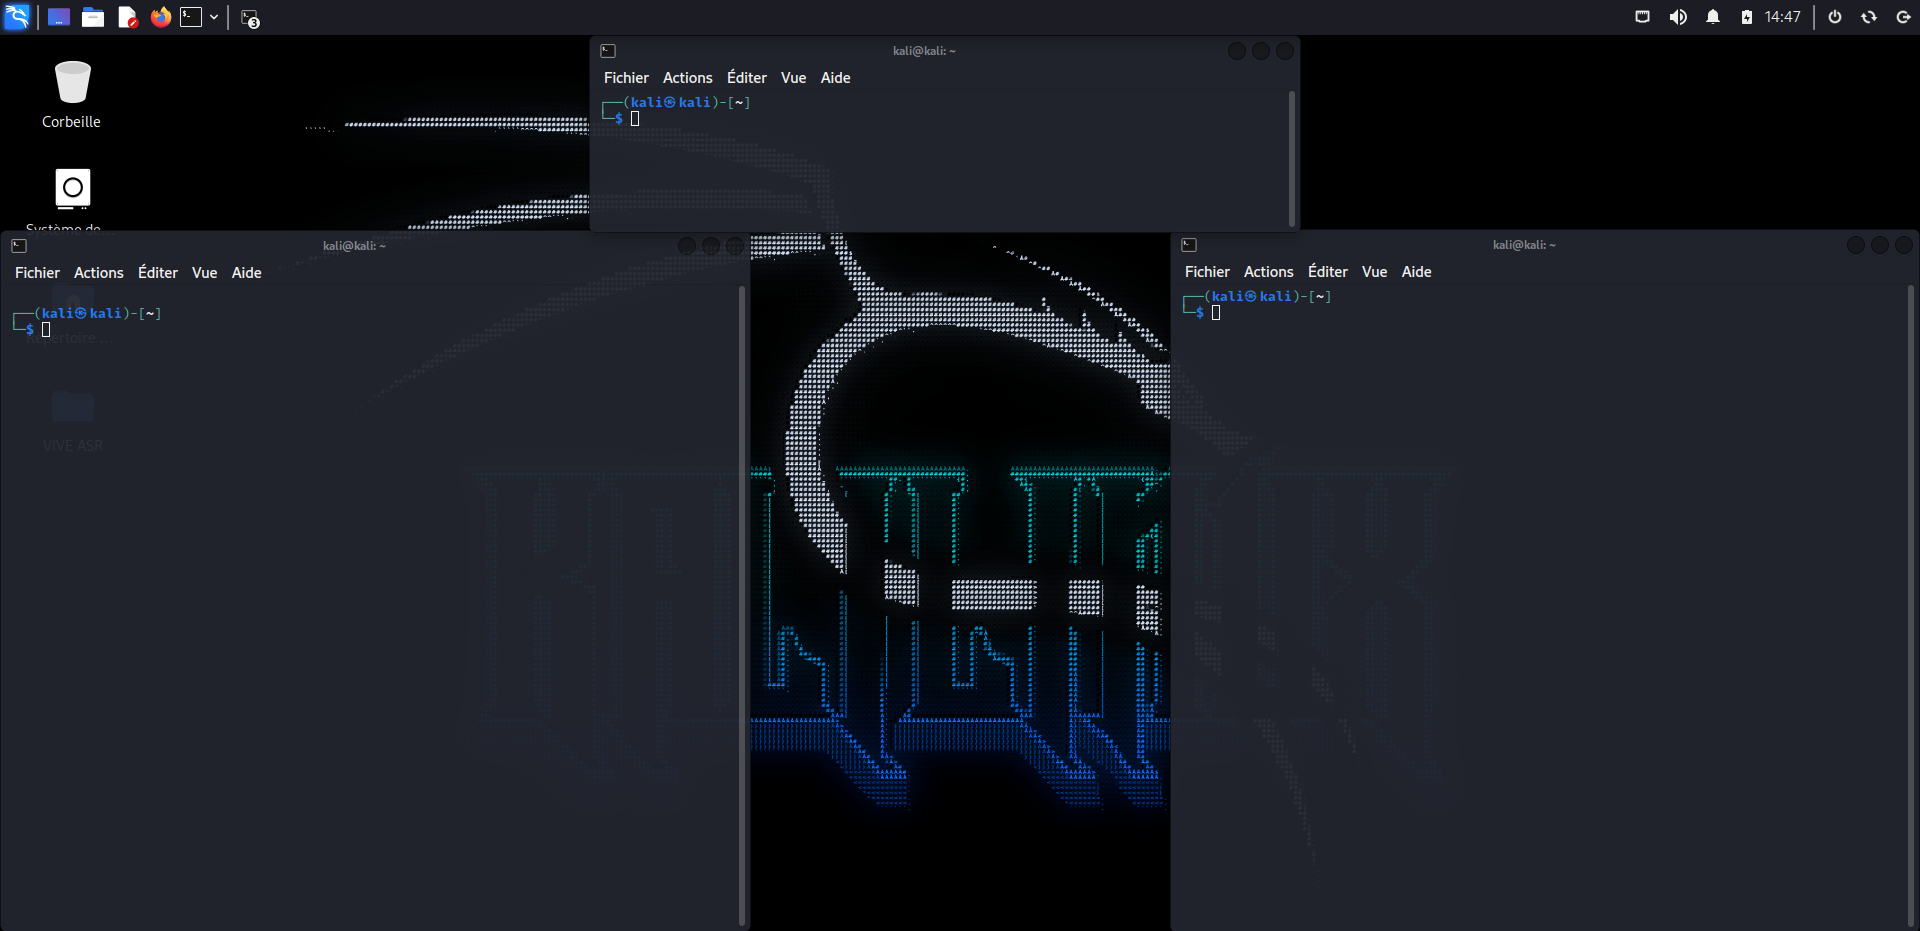
\includegraphics[width=\paperwidth,height=\paperheight]{Virt.png}}
\end{document}
